\section{Soluzione di sistemi LTI (Linear Time-Invariant) continui nel tempo}
\subsection{Come si imposta la soluzione di un sistema LTI continuo?}
Consideriamo un sistema LTI continuo rappresentato in forma stato-spazio:
\begin{equation}
    \begin{cases}
        \dot{x}(t) = A x(t) + B u(t) \\
        y(t) = C x(t) + D u(t)
    \end{cases}
\end{equation}
Dove $A$, $B$, $C$ e $D$ sono matrici di dimensioni opportune. La matrice $A$ è detta matrice di stato, $B$ è la matrice di ingresso, $C$ è la matrice di uscita e $D$ è la matrice di feedthrough (o matrice di trasmissione diretta).
Per risolvere questo sistema, possiamo utilizzare la matrice esponenziale. La soluzione generale
La soluzione di un sistema LTI continuo è data dall'equazione di Lagrange:
\begin{equation}
    x(t) = e^{At} x(0) + \int_0^t e^{A(t-\tau)} B u(\tau) d\tau = x_{zi}(t) + x_{zs}(t)
\end{equation}
Dove $x_{zi}(t) = e^{At} x(0)$ è la soluzione del sistema omogeneo (ovvero la soluzione senza ingresso)[risposta libera dello stato] e $x_{zs}(t) = \int_0^t e^{A(t-\tau)} B u(\tau) d\tau$ è la soluzione particolare (ovvero la soluzione dovuta all'ingresso)[risposta forzata dello stato].
La computazione di $x(t)$ e $y(t)$ attraverso la trasformata di Laplace è un metodo ottenuto attraverso il seguente schema:
\begin{center}
    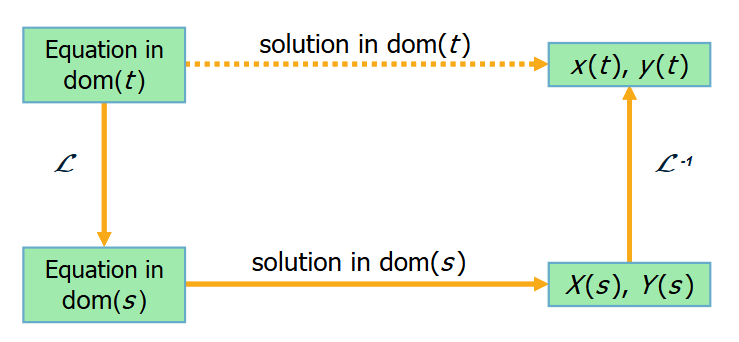
\includegraphics[width=0.8\textwidth]{foto/cph3/1.png}
\end{center}